\documentclass[12pt,twocolumn]{IEEEtran11}

\usepackage{times}
\usepackage{epsfig}
\usepackage[T1]{fontenc}
\usepackage{graphicx}
\usepackage{subfigure}
\def\BibTeX{{\rm B\kern-.05em{\sc i\kern-.025em b}\kern-.08em
    T\kern-.1667em\lower.7ex\hbox{E}\kern-.125emX}}

\oddsidemargin -15pt
\evensidemargin -15pt
\leftmargin 0 pt
\topmargin -30pt
\textwidth = 6.9 in
\textheight = 9.0 in

\newcommand{\itembase}{\setlength{\itemsep}{0pt}}
\newcommand{\eg}{{\it e.g., }}
\newcommand{\ie}{{\it i.e., }}
\graphicspath{{FIG/}}

\begin{document}
\bibliographystyle{IEEE}

\title{\Large \bf A Receiver-driven Framework for Peer-to-Peer Streaming
%\thanks{
}
\author{
John Doe\\
Information and Computer science Department\\
University of Oregon\\
{\em john@cs.uoregon.edu}
}
\maketitle
% You have to do this to suppress page numbers.  Don't ask.
%\pagestyle{empty}
\begin{abstract}
Write your abstract here
\end{abstract}

\begin{keywords} 
Quality Adaptive Streaming, Peer-to-Peer, Internet
\end{keywords}

\section{Introduction}
\label{sec:intro}
%\input{intro}
text for the intro should be added here. 
you can cite a refernce following this example,
TFRC \cite{Floyd:SIGCOMM00}. see main.tex for how this is done.

You can include a pdf figure in your paper as follows
\begin{figure}[t]
\centering
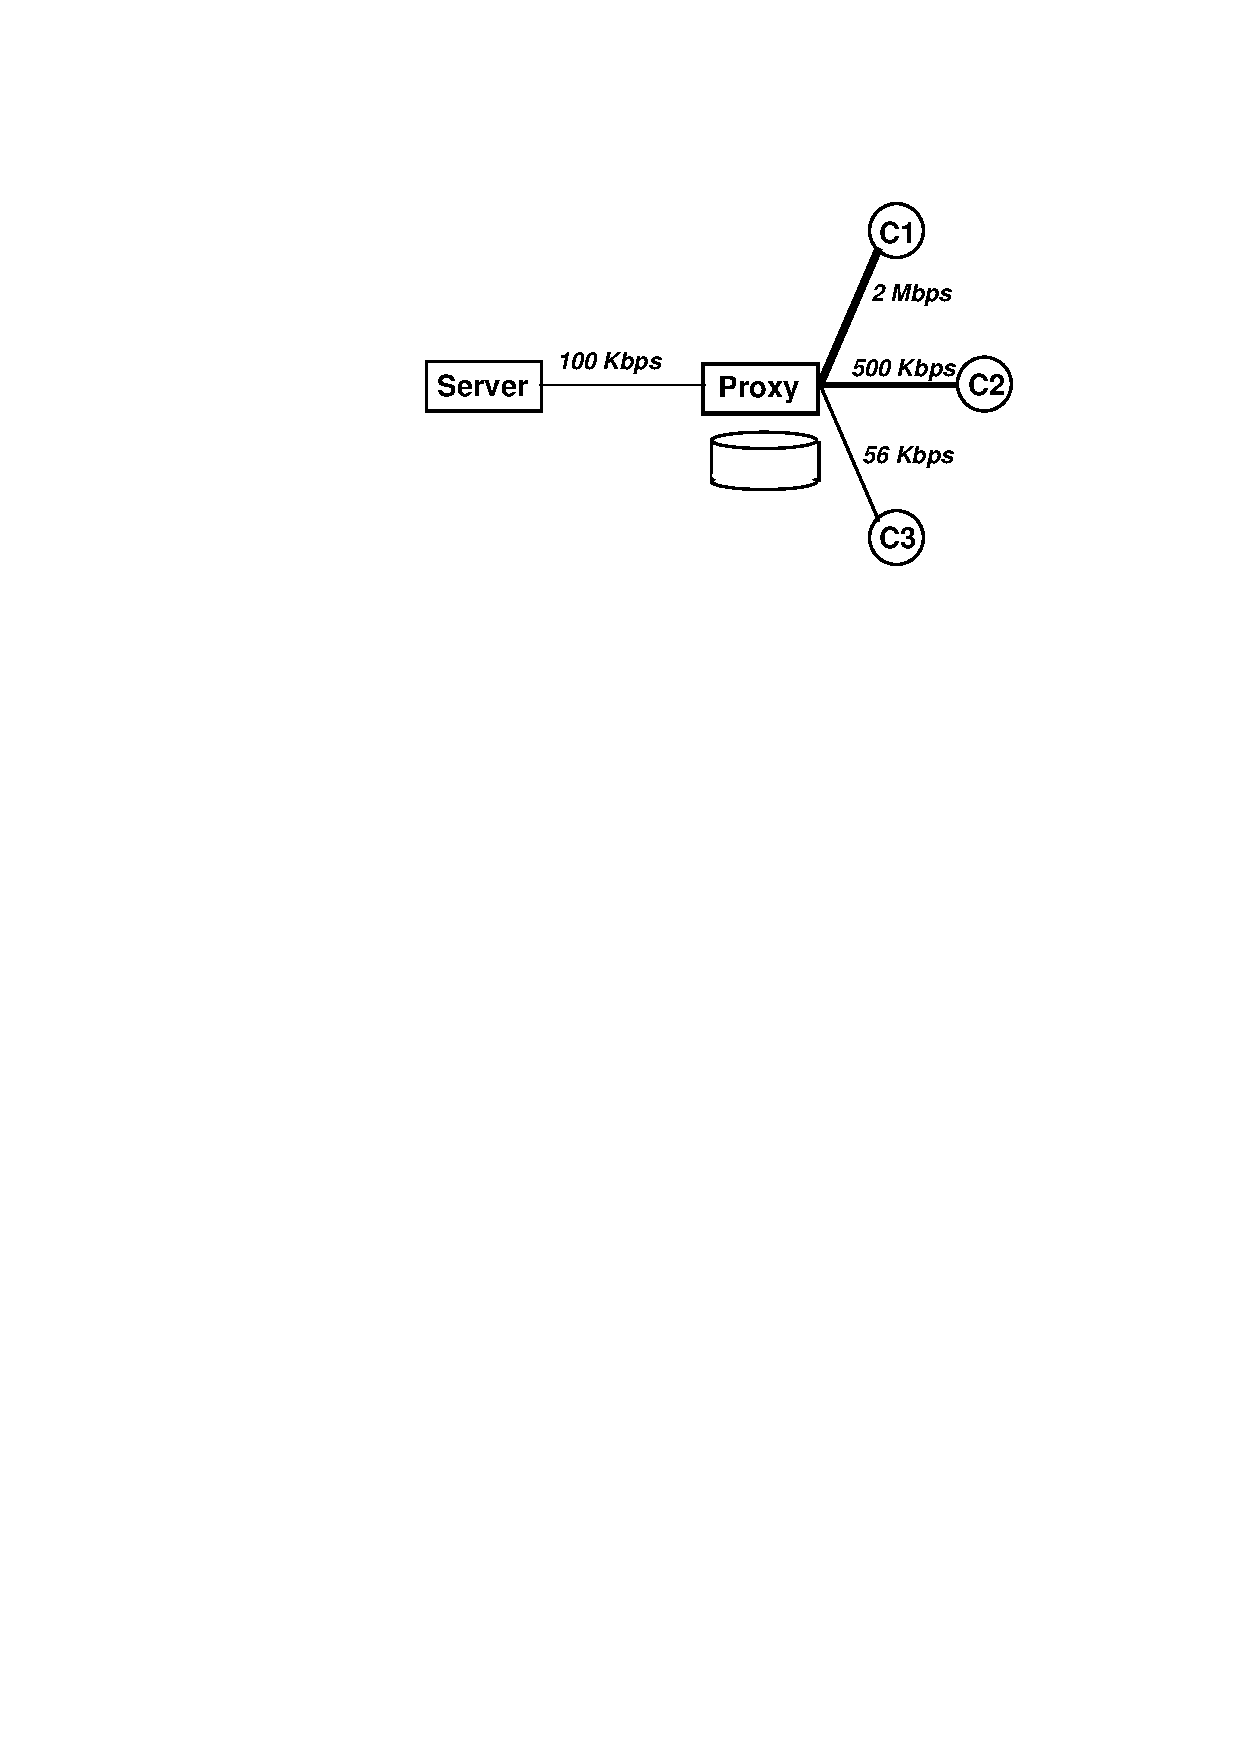
\includegraphics[width=1.0\textwidth]{mc.pdf}
\caption{Test}
\end{figure}


\subsection{Motivation}
text o fmotivation goes here

\subsubsection{Main Issues}
text of issues goes here

\section{Related Work}
\label{sec:rel-work}

\section{Framework: An Overview}
\label{sec:pals}

\section{Evaluation}
\label{sec:eval}

\section{Conclusions and Future Work}
\label{sec:-conc}

%% file citations.bib contains all the biblography
\bibliography{citations}
\end{document}
